\subsection{Stakeholderanalyse}\label{sec:stakeholderanalyse-teil-1}
\subsubsection{Identifizierung von Stakeholdern}
Um eine Analyse der Stakeholder durchführen zu können, müssen diese Stakeholder zuerst identifiziert werden.
Ein Stakeholder kann dabei dadurch beschrieben werden, dass er \gqq{eine Person oder eine Organisation [ist], die (direkt oder indirekt) Einfluss auf die Anforderungen des betrachteten Systems hat}\autocite[S. 8]{Maulhardt.a}.
Um diese Personen und Organisationen zu identifizieren, gibt es verschiedene Methoden.

Zuerst sollte Brainstorming genutzt werden, um möglichst viele Stakeholder zu identifizieren.
Dazu wird insbesondere mit Personen geredet, welche direkt mit dem Projekt zu tun haben beziehungsweise damit zu tun haben werden.
Als Ergebnis entsteht eine erste Liste mit möglichen Stakeholdern, welche allerdings noch nicht dem Anspruch der Vollständigkeit gerecht werden kann.

Um die Liste der Stakeholder zu vervollständigen, kann nun mit der Analyse von vorhandenen Dokumenten begonnen werden.
Dabei werden alle Dokumente, welche mit dem Projekt zu tun haben, durchsucht und nach Stakeholdern ermittelt.
Vornehmlich Verträge, die mit dem Projekt zu tun haben, bieten dabei einen guten Anhaltspunkt, da hier bereits Stakeholder genannt werden können.

Zuletzt ist eine Analyse der Produktentwicklung zu empfehlen.
Dabei können verschiedene Aspekte des Prozesses betrachtet werden, um Stakeholder zu identifizieren, indem man sich die folgenden Fragen stellt:

\begin{itemize}
    \item \textbf{Entwicklungsschritte:} Wer ist an den einzelnen Schritten der Entwicklung beteiligt?
    \item \textbf{Ressourcen:} Welche Ressourcen werden benötigt und wer stellt diese bereit?
    \item \textbf{Abhängigkeiten:} Welche Abhängigkeiten hat das Projekt von anderen Projekten beziehungsweise von anderen Personengruppen?
    \item \textbf{Ergebnisse:} Wer ist an den Ergebnissen des Projekts interessiert?
\end{itemize}

Die Stakeholder unterscheiden sich natürlich stark bei unterschiedlichen Projekten.
Allerdings kann gesagt werden, dass die Benutzer des Produkts sowie die Erwerber quasi ein minimales Set an Stakeholdern darstellen.
Zwei weitere Gruppen stellt zum einen die Organisation, welche das Produkt entwickelt und zum anderen regulatorische Behörden dar\autocite[vgl.][S. 8]{ISONorm.a}.

\subsubsection{Analyse der Stakeholder}
Nachdem die Stakeholder identifiziert wurden, können diese nun analysiert werden.
Dabei werden die Stakeholder nach verschiedenen Kriterien eingeteilt, um die Bedeutung der Stakeholder für das Projekt zu ermitteln.

Eine übliche Methode ist die Einordnung der Stakeholder in die Power-Interest Matrix, welche von Aubrey Mendelow entwickelt wurde.
Diese Matrix stellt die Stakeholder in Abhängigkeit von ihrer Macht und ihrem Interesse an dem Projekt dar\autocite[vgl.][S. 6f]{Botten.2006}.

\begin{figure}[ht]
    \centering
    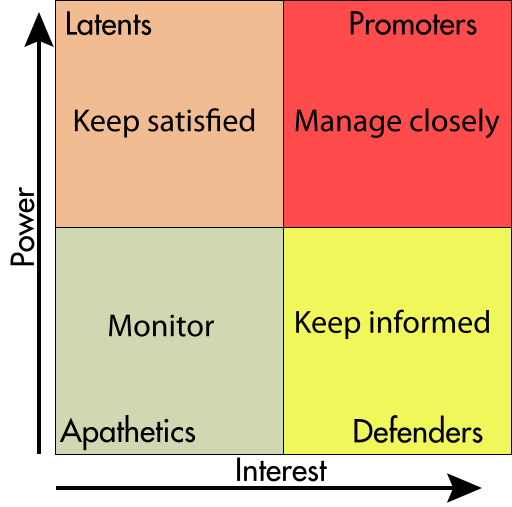
\includegraphics[width=0.3\textwidth]{Stakeholders_matrix}
    \caption{Power-Interest Matrix von Aubrey Mendelow}
    \label{fig:power-interest-matrix1}
\end{figure}

Mit diesen vier verschiedenen Gruppen muss jeweils unterschiedlich umgegangen werden.

\begin{itemize}
    \item \textbf{Apathetics:} Durch den geringen Einfluss und die geringe Macht ist diese Gruppe leicht zu überzeugen, weshalb sie eine eher geringe Beachtung finden.
    \item \textbf{Defenders:} Diese Gruppe ist zwar nicht besonders stark, hat aber ein starkes Interesse an dem Projekt.
        Da diese Gruppe es auch schaffen kann, Gruppen mit mehr Einfluss zu überzeugen, sollten diese Stakeholder in die Prozesse eingeschlossen werden und dadurch davon überzeugt werden, dass das Projekt für sie von Vorteil ist.
    \item \textbf{Latents:} Da diese Gruppe zwar viel Einfluss hat, aber kein Interesse an dem Projekt hat, sollte verhindert werden, dass diese Gruppe zu Promotern wird.
        Dies kann durch eine gute Kommunikation erreicht werden, um die Vorteile des Projekts zu verdeutlichen.
    \item \textbf{Promoters:} Bei dieser Gruppe muss unterschieden werden, ob diese dem Projekt positiv oder negativ gegenübersteht.
        In beiden Fällen ist es allerdings notwendig, durch ausreichend Lehre/Kommunikation diese Gruppe zu überzeugen, dass das Projekt notwendig ist.
        Anschließend sollte auch mit dieser Gruppe diskutiert werden, wie man das Projekt am besten umsetzt, um auch deren Eindrücke in das Projekt einfließen zu lassen.
\end{itemize}

Eine weitere Methode zur Einordnung der verschiedenen Stakeholder ist das Hervorhebungs-Modell von Ronald Mitchell, Bradley Agle und Donna Wood.
Dieses Modell unterscheidet zwischen acht verschiedenen Arten von Stakeholdern, welche unterschiedliche Bedeutung für das Projekt haben.
Diese Unterscheidung wird durch eine Einordnung in Kategorien Power, Legitimität und Dringlichkeit vorgenommen.
Dabei wird analysiert, wie viele von den genannten Kategorien auf die einzelnen Stakeholder zutreffen.

\begin{figure}[ht]
    \centering
    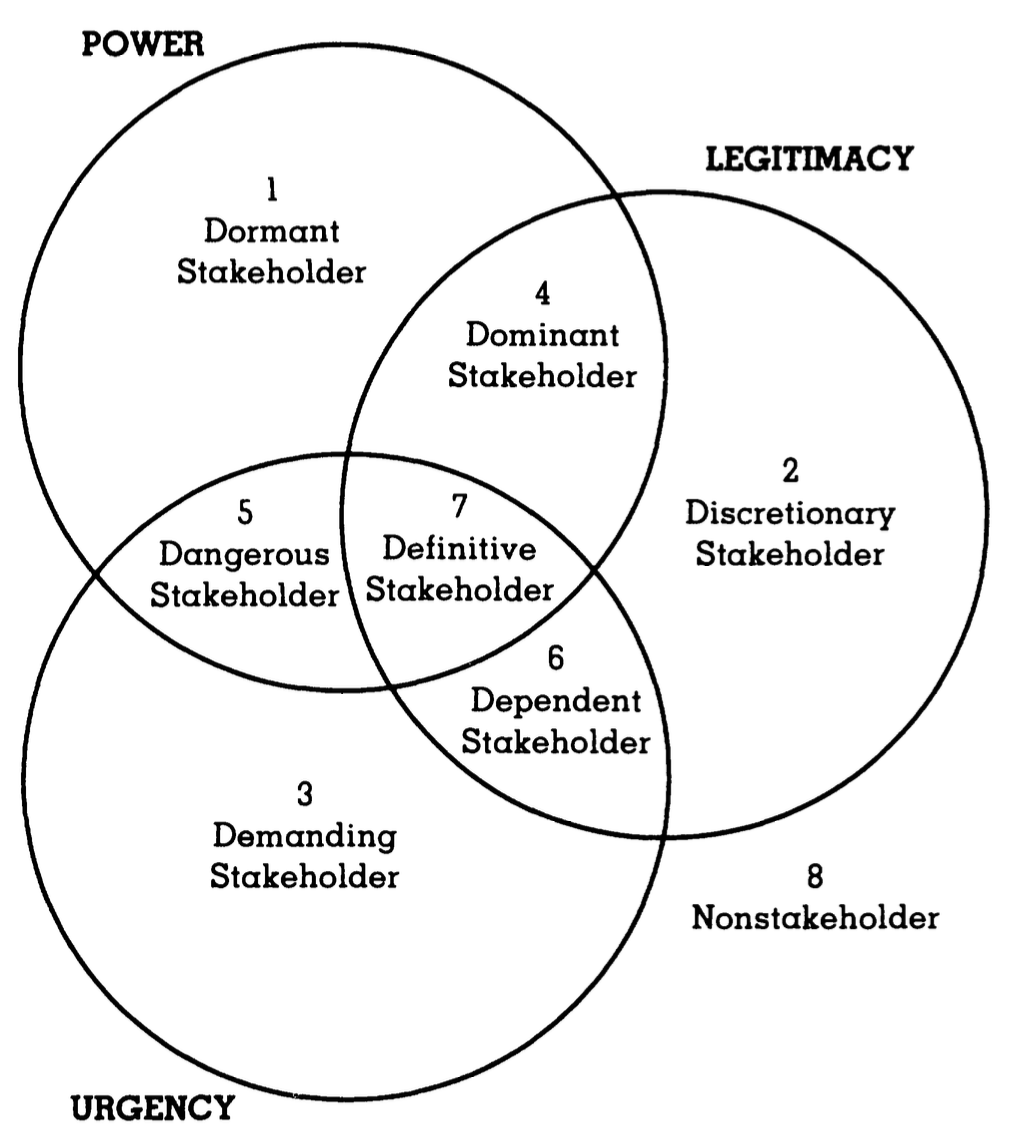
\includegraphics[width=0.3\textwidth]{Salience-Model}
    \caption{Hervorhebungs-Modell von Ronald Mitchell, Bradley Agle und Donna Wood\autocite[S. 874]{Mitchell.1997}}
    \label{fig:highlight-model}
\end{figure}

Personengruppen, auf die eine von den drei Kategorien zutrifft, werden als latent eingestuft.
Diese müssen aufgrund ihrer begrenzten Zeit, Energie und anderer Ressourcen vom Management nicht unbedingt berücksichtigt werden.

Personengruppen, auf die zwei von den drei Kategorien zutreffen, werden als potenziell wichtig eingestuft.
Diese sogenannten \gqq{erwartenden} Stakeholder sind aktiv und haben ein Interesse an dem Projekt.
Dementsprechend sollte der Austausch zwischen den Projektleitern und diesen Stakeholdern intensiviert werden.

Die wichtigsten Stakeholder sind diejenigen, auf die alle drei Kategorien zutreffen.
Dabei ist auch darauf zu achten, ob erwartende Stakeholder zu dieser Gruppe aufsteigen, da nur ein Attribut fehlt, um dieser Gruppe zugeordnet zu werden.
Mit diesen sollte ein intensiver Austausch gepflegt werden und auf Anmerkungen dieser Gruppe mit entsprechender Priorität reagiert werden\autocite[vgl.][S. 874ff]{Mitchell.1997}.
